\section{Implementierung SmBasic}

Der DEA der ersten Implementierung wird im Folgenden als SmBasic bezeichnet. Dieser DEA soll das grundlegende Prinzip des Saga-Patterns unter Verwendung der Backward-Recovery implementieren. Jeglicher Fehler führt dazu, dass die SEC eine Kompensierung der Saga verfolgt.

\subsection{Strategie für die Konstruierung des DEAs SmBasic}

Alle Erfolge eines Ts führen zum folgenden T. Alle anderen Ergebnisse führen für Ts zu einem Zustandswechsel zu dem nächstkleineren C. Erfolgreiche Cs führen zum nächstkleinerem C. Alle anderen Ergebnisse führen für Cs zu einem Zustandswechsel in den Zustand \textit{FailedWithCompensation}. Das letzte T führt bei Erfolg zu einem Übergang in den Zustand \textit{Done}. Ebenso führt $C_1$ bei Erfolg zu einem Übergang in den Zustand \textit{FailedWithCompensation}. 

\begin{center}
	\begin{longtable}[h]{|p{2.6cm}|p{2cm}|p{2.8cm}|p{5cm}|}
		\hline
		Ergebnistyp & Zustand & Ergebnis $e$& Folgezustand \\ \hline
		API-Ergebnis & $T_n$ & $e \in \{Tn_{200}\}$ & $T_{n+1}$ \\ \hline
		API-Ergebnis & $T_n$ & $e \not\in \{Tn_{200}\}$ & $C_{n-1}$ \\ \hline
		IPE & $T_n$ & $e \in \{Tn_{Success}\}$ & $T_{n+1}$\\ \hline
		IPE & $T_n$ & $e \not\in \{Tn_{Success}\}$ & $C_{n-1}$\\ \hline
		API-Ergebnis & $C_n$ & $e \in \{Cn_{200}\}$ & $C_{n-1}$ \\ \hline
		API-Ergebnis & $C_n$ & $e \not\in \{Cn_{200}\}$ & \textit{FailedWithoutCompensation} \\ \hline
		IPE & $C_n$ & $e \in \{Cn_{Success}\}$ & $C_{n-1}$\\ \hline
		IPE & $C_n$ & $e \not\in \{Cn_{Success}\}$ & \textit{FailedWithoutCompensation}\\ \hline
	\end{longtable}
\end{center}
\FloatBarrier

Aus diesem Regelwerk ergibt sich der in \cref{fig:fig_sm_basic} dargestellte DEA. 

\begin{figure}[H]
	\centering
	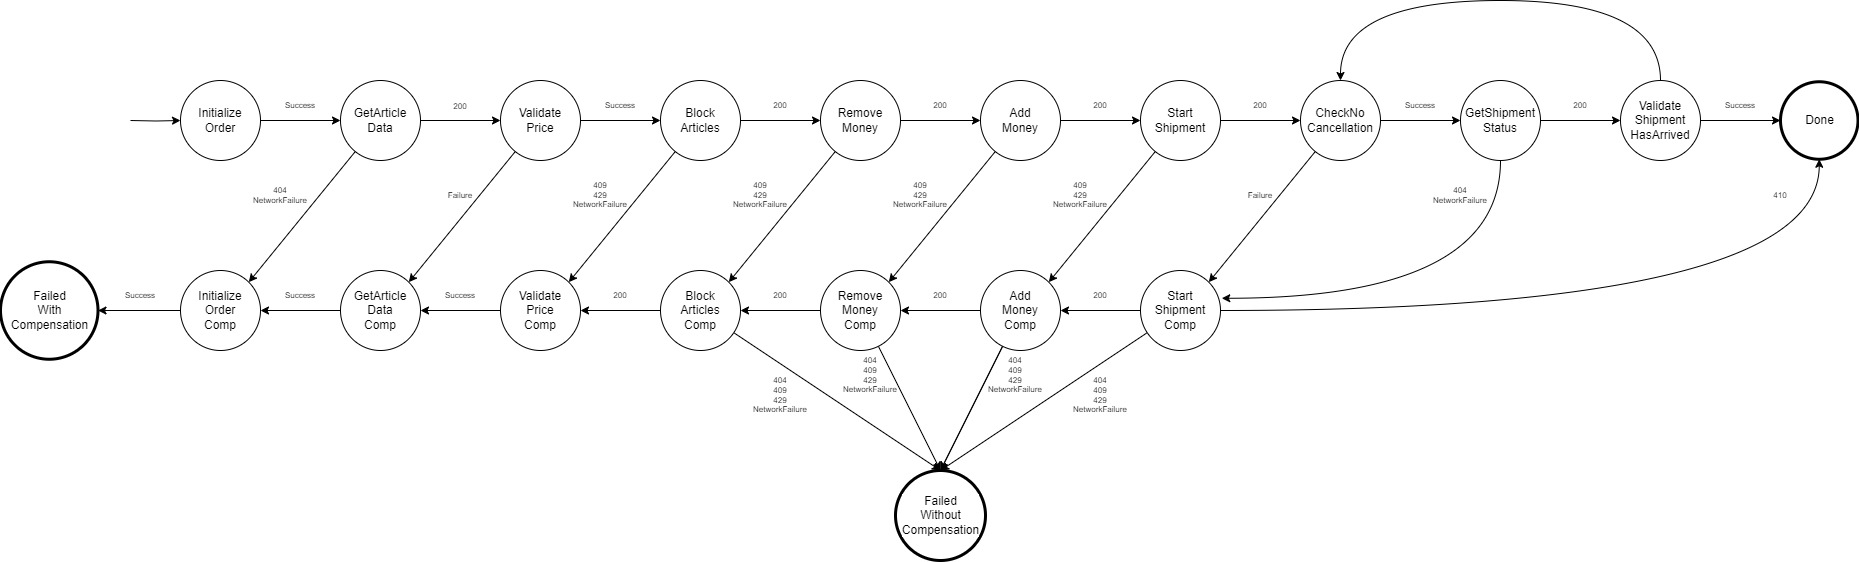
\includegraphics[width=\linewidth]{figures/ChapterVersuchsdurchführung/sm_basic.jpg}
	\caption{DEA für SmBasic}
	\label{fig:fig_sm_basic}
\end{figure}
\FloatBarrier

\subsection{StateAnalysisResult}

\paragraph*{Testfall FinishOrders} \mbox{}\\
Folgende Tabelle bildet das StateAnalysisResult der Messung des SmBasic in Testfall FinishOrders.

\begin{center}
	\fontsize{9}{12}\selectfont
	\begin{longtable}[h]{|p{5cm}|p{1cm}|p{1cm}|p{1cm}|}
		\hline
		Messwert & S1 & S2 & S3 \\ \hline
		\endhead
		%\label{tab:smbasic_stateanalysisresult_finishorders}
		\endfoot
		successfull\-Percentage & 0.80 & 0.42 & 0.19 \\ \hline
		finished\-Percentage & 1.0 & 1.0 & 1.0 \\ \hline
		pending\-Percentage & 0.0 & 0.0 & 0.0 \\ \hline
		failedWithCompensation\-Percentage & 0.20 & 0.53 & 0.72 \\ \hline
		failedWithoutCompensation\-Percentage & 0.0 & 0.06 & 0.10 \\ \hline
		hasCorrectEndstate\-Percentage & 0.80 & 0.42 & 0.19 \\ \hline
		containsAllExpectedLogs\-Percentage & 0.80 & 0.38 & 0.15 \\ \hline
		isSuccessfullTestInstance\-Percentage & 0.80 & 0.38 & 0.15 \\ \hline
	\end{longtable}
\end{center}
\FloatBarrier

Die Messung zeigt, dass bereits in Testszenario 1 nur 80\% der Sagas zum erwarteten Endzustand führen. Der Anteil der Sagas, die den Zustand \textit{Success} erreichen, wird mit jedem Testszenario geringer: 80\% in Testszenario S1, 42\% in S2 und 19\% in S3.

Das ist damit zu begründen, dass jeglicher Fehler in der Ausführung des SmBasic zur Kompensierung führt. Zu den Fehlern, die zur Kompensierung (für Ts) oder zum Zustand \textit{FailedWithoutCompensation} (für Cs) führen, gehören neben den Fehlern, die einen kritischen Konflikt ausdrücken auch vorübergehende Fehler (API-Ergebnisse mit $tn_{429}$) und in S2 und S3 Netzwerkfehler. 

Dies drückt sich außerdem in dem Messwert \textit{failedWithoutCompensation} aus, der ebenfalls in jedem Testszenario größer wird.

In \cref{tab:transaktionslog_ts1_tc1_429} ist das Transaktionslog einer Saga abgebildet, die aufgrund eines vorübergehenden Fehlers abgebrochen wurde. 

\begin{center}
	\fontsize{9}{12}\selectfont
	\begin{longtable}[h]{|p{4.5cm}|p{7cm}|}
		\hline
		Zustand & Ergebnis \\* \hline
		\endhead
		\hline
		\caption{Transaktionslog für Saga im Testfall 1 und Testszenario 1}
		\label{tab:transaktionslog_ts1_tc1_429}
		\endfoot
  		InitializeOrder & InitializeSagaSuccess \\* \hline
		GetArticleData & GetProductData200 \\* \hline
		ValidatePrice & ValidatePriceSuccess \\* \hline
		\rowcolor{Gray}
		BlockArticles & BlockArticles429 \\* \hline
		ValidatePriceCompensation & ValidatePriceCompensationSuccess \\* \hline
		GetArticleDataCompensation & GetProductDataCompensationSuccess \\* \hline
		InitializeOrderCompensation & InitializeSagaCompensationSuccess \\* \hline
	\end{longtable}
\end{center}
\FloatBarrier

\paragraph*{Testfall CancelOrders} \mbox{}\\
In \cref{tab:smbasic_stateanalysisresult_cancelorders} ist das StateAnalysisResult für den Testfall CancelOrders dargestellt. Hier zeigt sich die Berechtigung des Messwertes \textit{isSuccessfullTestInstancePercentage}. Der erwartete Endzustand \textit{FailedWithCompensation} wird in diesem Testfall erwartet und in Testszenario 1 in 95\% aller Sagas erreicht. Der Messwert \textit{containsAllExpectedLogsPercentage} zeigt, dass in Testszenario 1 lediglich 87\% die erwarteten Logs enthalten. Das bedeutet, dass ein Anteil der Sagas mit Endzustand \textit{FailedWithCompensation} aufgrund eines Fehlers zur Kompensierung gewechselt haben und nicht wie erwartet den Zustand \textit{CheckNoCancellation} erreicht haben. Somit stellen diese Sagas keine erfolgreichen Testinstanzen mehr dar.

\begin{center}
	\fontsize{9}{12}\selectfont
	\begin{longtable}[h]{|p{5cm}|p{1cm}|p{1cm}|p{1cm}|}
		\hline
		Messwert & S1 & S2 & S3 \\ \hline
		\endhead
		%\label{tab:smbasic_stateanalysisresult_cancelorders}
		\endfoot
		successfull\-Percentage & 0.0 & 0.0 & 0.0 \\ \hline
		finished\-Percentage & 1.0 & 1.0 & 1.0 \\ \hline
		pending\-Percentage & 0.0 & 0.0 & 0.0 \\ \hline
		failedWithCompensation\-Percentage & 0.95 & 0.77 & 0.75 \\ \hline
		failedWithoutCompensation\-Percentage & 0.05 & 0.23 & 0.25 \\ \hline
		hasCorrectEndstate\-Percentage & 0.95 & 0.77 & 0.75 \\ \hline
		containsAllExpectedLogs\-Percentage & 0.87 & 0.27 & 0.06 \\ \hline
		isSuccessfullTestInstance\-Percentage & 0.87 & 0.27 & 0.06 \\ \hline
	\end{longtable}
\end{center}
\FloatBarrier

\paragraph*{Abgebrochene Sagas} \mbox{}\\
Der Messwert \textit{failedWithoutCompensationPercentage} stellt den Anteil der Sagas dar, die aufgrund eines Fehlers während einer Kompensierung die Ausführung abbrechen. Im konstruierten SmBasic gibt es keine Retries. Das bedeutet, dass jede Saga, die zwei fehlerhafte Ergebnisse im Log enthält, in diesem Zustand landet. Ein Beispiel dafür ist im Transaktionslog in \cref{tab:transaktionslog_ts2_cancelorders_smbasic} abgebildet. 

\begin{center}
	\fontsize{9}{12}\selectfont
	\begin{longtable}[h]{|p{4.5cm}|p{7cm}|}
		\hline
		Zustand & Ergebnis \\* \hline
		\endhead
		\hline
		\caption{Transaktionslog für Saga im Testfall CancelOrders und Testszenario 2}
		\label{tab:transaktionslog_ts2_cancelorders_smbasic}
		\endfoot
		InitializeOrder &  InitializeSagaSuccess \\* \hline
		GetArticleData &  GetProductData200 \\* \hline
		ValidatePrice &  ValidatePriceSuccess \\* \hline
		BlockArticles &  BlockArticles200 \\* \hline
		RemoveMoney &  RemoveMoney200 \\* \hline
		AddMoney &  AddMoney200 \\* \hline
		StartShipment &  StartShipment200 \\* \hline
		CheckNoCancellation &  CheckNoCancellationSuccess \\* \hline
		GetShipmentStatus &  GetShipmentStatus200 \\* \hline
		\rowcolor{Gray}
		ValidateShipmentHasArrived &  ShipmentHasArrivedFailure \\* \hline
		CheckNoCancellation &  CheckNoCancellationSuccess \\* \hline
		GetShipmentStatus &  GetShipmentStatusNetworkFailure \\* \hline
		StartShipmentCompensation &  StartShipmentCompensation200 \\* \hline
		\rowcolor{Gray}
		AddMoneyCompensation &  AddMoneyCompensationNetworkFailure \\* \hline
	\end{longtable}
\end{center}
\FloatBarrier

\subsection{TransactionAnalysisResult}
In \cref{tab:smbasic_stateanalysisresult} sind die TransactionAnalysisResults für beide Testfälle dargestellt. 

\begin{center}
	\fontsize{9}{12}\selectfont
	\begin{longtable}[h]{|p{5cm}|p{1cm}|p{1cm}|p{1cm}|}
		\hline
		 & S1 & S2 & S3 \\ \hline
		\endhead
		%\label{tab:smbasic_stateanalysisresult}
		\endfoot
		FinishOrders & 1 & 1 & 0.87\\ \hline	
		CancelOrders & 1 & 1 & 0.81\\ \hline
	\end{longtable}
\end{center}
\FloatBarrier

In beiden Testfällen treten unter den Bedingungen von Testszenario 1 und 2 keine Inkonsistenzen auf. In Testszenario 3 führen 87\% im Testfall \textit{FinishOrders} und 81\% im Testfall \textit{CancelOrders} aller Sagas zu mindestens zu einem inkonsistenten Zustand innerhalb der Teilnehmerservices. 

Neben den Sagas, die im Endzustand \textit{FailedWithoutCompensation} landen, führen auch Sagas zu einem inkonsistenten Systemzustand, die nach einem Netzwerkfehler mit der Kompensierung fortfahren. Ein Beispiel dafür ist das Transaktionslog in \cref{tab:transaktionslog_cancelorders_ts3}. Der BankService hat die lokale Transaktion \textit{RemoveMoney} erfolgreich ausgeführt. Die Response ging verloren, weshalb der Koordinator mit der Kompensierung fortgefahren hat. Die lokale Transaktion \textit{RemoveMoney} wurde nicht kompensiert. Fachlich stellt dieses Saga-Log einen Bestellprozess dar, der abgebrochen wurde. Das Geld des Kundenkontos wurde abgebucht und nicht rückerstattet. Der Saga-Prozess hat keine Kenntnis von diesem fachlichen Fehler.

\begin{center}
	\fontsize{9}{12}\selectfont
	\begin{longtable}[h]{|p{4.5cm}|p{5.5cm}|}
		\hline
		Zustand & Ergebnis \\* \hline
		\endhead
		\caption{Transaktionslog einer Saga für \textit{CancelOrders} im Testszenario 3}
		\label{tab:transaktionslog_cancelorders_ts3}
		\endfoot
		InitializeOrder & InitializeSagaSuccess \\ \hline
		GetArticleData & GetProductData200 \\ \hline
		ValidatePrice & ValidatePriceSuccess \\ \hline
		BlockArticles & BlockArticles200 \\ \hline
		\rowcolor{Gray}
		RemoveMoney & RemoveMoneyNetworkFailure \\ \hline
		\rowcolor{Gray}
		BlockArticlesCompensation & BlockArticlesCompensation200 \\ \hline
		ValidatePriceCompensation & ValidatePriceCompensationSuccess \\ \hline
		GetArticleDataCompensation & GetProductDataCompensationSuccess \\ \hline
		InitializeOrderCompensation & InitializeSagaCompensationSuccess \\ \hline
	\end{longtable}
\end{center}
\FloatBarrier
